\documentclass{beamer}
\mode<presentation> {
	
	% The Beamer class comes with a number of default slide themes
	% which change the colors and layouts of slides. Below this is a list
	% of all the themes, uncomment each in turn to see what they look like.
	
	%\usetheme{default}
	%\usetheme{AnnArbor}
	%\usetheme{Antibes}
	%\usetheme{Bergen}
	%\usetheme{Berkeley}
	%\usetheme{Berlin}
	%\usetheme{Boadilla}
	%\usetheme{CambridgeUS}
	%\usetheme{Copenhagen}
	%\usetheme{Darmstadt}
	%\usetheme{Dresden}
	%\usetheme{Frankfurt}
	%\usetheme{Goettingen}
	%\usetheme{Hannover}
	%\usetheme{Ilmenau}
	%\usetheme{JuanLesPins}
	%\usetheme{Luebeck}
	\usetheme{Madrid}
	%\usetheme{Malmoe}
	%\usetheme{Marburg}
	%\usetheme{Montpellier}
	%\usetheme{PaloAlto}
	%\usetheme{Pittsburgh}
	%\usetheme{Rochester}
	%\usetheme{Singapore}
	%\usetheme{Szeged}
	%\usetheme{Warsaw}
	
	% As well as themes, the Beamer class has a number of color themes
	% for any slide theme. Uncomment each of these in turn to see how it
	% changes the colors of your current slide theme.
	
	%\usecolortheme{albatross}
	%\usecolortheme{beaver}
	%\usecolortheme{beetle}
	%\usecolortheme{crane}
	%\usecolortheme{dolphin}
	%\usecolortheme{dove}
	%\usecolortheme{fly}
	%\usecolortheme{lily}
	%\usecolortheme{orchid}
	%\usecolortheme{rose}
	%\usecolortheme{seagull}
	%\usecolortheme{seahorse}
	%\usecolortheme{whale}
	%\usecolortheme{wolverine}
	
	%\setbeamertemplate{footline} % To remove the footer line in all slides uncomment this line
	%\setbeamertemplate{footline}[page number] % To replace the footer line in all slides with a simple slide count uncomment this line
	
	%\setbeamertemplate{navigation symbols}{} % To remove the navigation symbols from the bottom of all slides uncomment this line
}

\usepackage{graphicx} % Allows including images
\usepackage{booktabs} % Allows the use of \toprule, \midrule and \bottomrule in tables
\usepackage[utf8]{inputenc}
\usepackage[english,frenchb]{babel}
\usepackage[Algorithme]{algorithm}
\usepackage{algorithmic}
\usepackage{ulem}
\newcommand\redout{\bgroup\markoverwith
	{\textcolor{red}{\rule[0.5ex]{2pt}{0.8pt}}}\ULon}
\usepackage{tikz}
\usetikzlibrary{arrows}
\usetikzlibrary{calc,shapes,patterns}
\newcommand{\tikzmark}[1]{\tikz[overlay,remember picture] \node (#1) {};}
\def\checkmarkg{\tikz\fill[scale=0.4,black!30!green](0,.35) -- (.25,0) -- (1,.7) -- (.25,.15) -- cycle;}
\def\checkmarky{\tikz\fill[scale=0.4,black!30!yellow](0,.35) -- (.25,0) -- (1,.7) -- (.25,.15) -- cycle;}
\usepackage{amssymb}% http://ctan.org/pkg/amssymb
\usepackage{pifont}% http://ctan.org/pkg/pifont
\usepackage{color}
\usepackage{filecontents}
\usepackage{soul}
\usepackage{bibentry}
\usepackage{booktabs} % Allows the use of \toprule, 

\newcommand{\xmark}{\ding{55}}%
\newcommand\tab[1][1cm]{\hspace*{#1}}
\setbeamertemplate{items}[circle]

\newcommand\mynum[1]{%
	\usebeamercolor{enumerate item}%
	\tikzset{beameritem/.style={circle,inner sep=0,minimum size=2ex,text=enumerate item.bg,fill=enumerate item.fg,font=\footnotesize}}%
	\tikz[baseline=(n.base)]\node(n)[beameritem]{#1};%
}

\usepackage{caption}
\captionsetup{font=scriptsize,labelfont=scriptsize}

\makeatletter
\setbeamertemplate{headline}{%
	\begin{beamercolorbox}[ht=2.25ex,dp=3.75ex]{section in head/foot}
		\insertnavigation{\paperwidth}
	\end{beamercolorbox}%
}%
\makeatother
\newcommand{\CS}{\textsf{CS}}
\newcommand{\GPS}{\textsf{GPS}}
\newcommand{\GSS}{\textsf{GSS}}
\newcommand{\MADS}{\textsf{MADS}}
\newcommand{\IMFIL}{\textsf{IMFIL}}
\newcommand{\norm}[1]{\left\lVert#1\right\rVert}
\newcommand{\R}{\mathbb{R}}
%----------------------------------------------------------------------------------------
%	TITLE PAGE
%----------------------------------------------------------------------------------------

\title[Opportunisme et ordonnancement]{Opportunisme et ordonnancement en optimisation sans dérivées} % The short title appears at the bottom of every slide, the full title is only on the title page

\author{Loïc Anthony Sarrazin-Mc Cann} % Your name
\institute[GERAD] % Your institution as it will appear on the bottom of every slide, may be shorthand to save space
{
	École Polytechnique de Montréal \\ % Your institution for the title page
	\medskip
}
\date{\today} % Date, can be changed to a custom date

\begin{document}
	
\begin{frame}
	\titlepage % Print the title page as the first slide
\end{frame}

\begin{frame}
\frametitle{Gestion des contraintes : Barrière progressive}
$x^{feas}$ le meilleur point réalisable\\
$x^{inf}$ le meilleur point non-réalisable\\
\pause
La fonction de violation de contraintes : 
\begin{align*}
h(x) = \begin{cases}
\sum_{j\in J}^{}(\max(c_j(x),0))^2~ &\text{si}~x\in X\\
\infty~ &\text{sinon}
\end{cases}
\end{align*} 
\pause
\begin{figure}[h]
	\begin{center}
		\resizebox{.8\totalheight}{!}{
		\begin{tikzpicture}
		% Flèches
		\draw[->] (0,0) -- (8,0);
		\draw [->] (0,0) -- (0,5);
		% Axes 
		\draw (8,0) node[right] {$h$};
		\draw (0,5) node[above] {$f$};
		% Point faisable non domin
		\draw (0,3.5) node[]{$\bullet$};
		\draw (0,3.5) node[below left]{$x^{feas}$};
		%Point faisable dominé
		\draw (0,4.5) node[]{$\circ$};
		% Points non-dominés mais pas inf
		\draw (2,3.9) node[]{$\bullet$};
		\draw (4,1.7) node[]{$\bullet$};
		% Point non dominé inf
		\draw (6,0.7) node[]{$\bullet$};
		\draw (6,0.7) node[below left]{$x^{inf}$};
		% Points dominés
		\draw (2.9,4.2) node[]{$\circ$};
		\draw (5,1.7) node[]{$\circ$};
		\draw (6.6,1) node[]{$\circ$};
		\draw (7.5,0.5) node[]{$\circ$};
		% Droites délimitant zone réalisable
		\draw [-] (2,5) -- (2,3.9);
		\draw [-] (2,3.9) -- (4,3.9);
		\draw [-] (4,3.9) -- (4,1.7);
		\draw [-] (4,1.7) -- (6,1.7);
		\draw [-] (6,1.7) -- (6,0.7);
		\draw [-] (6,0.7) -- (7,0.7);
		% Droite pour h max
		\draw [-] (7,0) -- (7,5);
		\draw (7,0) node[below]{$h_{max}$};
		% Hachure de la région dominée
		\fill[pattern = north east lines,opacity = 0.5] (2,5) -- (2,3.9) -- (4,3.9) -- (4,1.7) -- (6,1.7) -- (6,0.7) -- (7,0.7) -- (7,0) -- (8,0) --(8,5) -- cycle;
		\end{tikzpicture}}
	\end{center}
	\caption{Barrière progressive, dominance et solutions courantes multiples} \label{fig:barrier}
\end{figure}
On veut minimiser $h(x)$ et $c(x)$
\end{frame}

%----------------------------------------------------------------------------------------
%	PRESENTATION SLIDES
%----------------------------------------------------------------------------------------

%------------------------------------------------
\section[Introduction]{Introduction} 
\tableofcontents[currentsection,currentsubsection,subsectionstyle=show/hide]
\subsection{Optimisation sans dérivées}
\begin{frame} %3
\frametitle{Optimisation sans dérivées}
\textbf{Problème d'optimisation} :
\begin{align*}
	\begin{cases}
		\underset{x\in \R^n}{\min} & f(x) \\
		\text{s.à.} & c_j(x) \leq 0 ~ ~ \forall j \in \{1,\dots,m\}\\
		~ & l_i \leq x_i \leq u_i ~ ~ \forall i \in \{1,\dots,n\}
	\end{cases}
\end{align*}
\begin{itemize}
	\pause
	\item $f(x)$ et $c_j(x)$ sont des boîtes noires.
\end{itemize}
\bigskip

\end{frame}
\begin{frame}%4
	\frametitle{Boîte noire}
	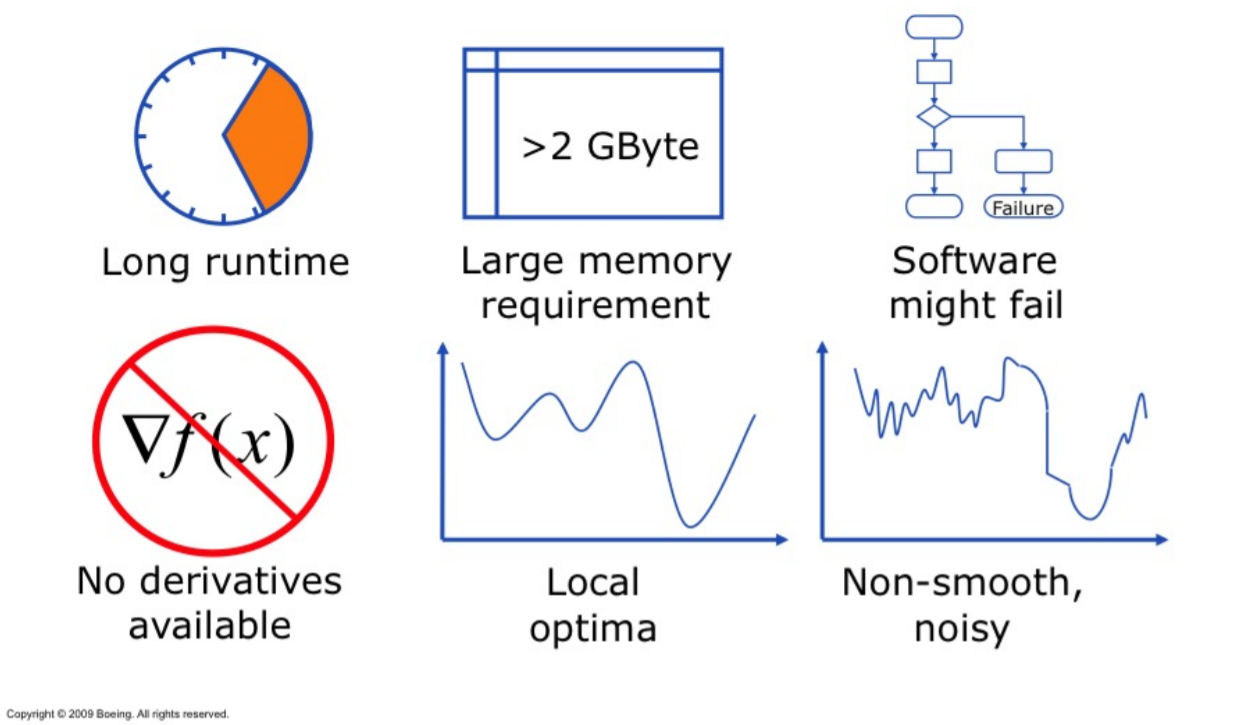
\includegraphics[width=\linewidth]{blackbox.png}
\end{frame}
\begin{frame}%5
\frametitle{Types d'algorithmes de DFO}
\textbf{Méthodes de région de confiance}
\smallskip
% Define block styles
%\tikzstyle{decision} = [diamond, draw, fill=blue!20, 
%text width=4.5em, text badly centered, node distance=3cm, inner sep=0pt]
\tikzstyle{block} = [rectangle, draw, fill=blue!20, 
text width=5em, text centered, rounded corners, minimum height=1em]
\tikzstyle{line} = [draw, -latex']
%
\begin{tikzpicture}[node distance = 6.3em, auto]
%% Place nodes
\node [block] (critic) {Criticalité};
\node [block, right of=critic] (step) {Calcul du pas};
\node [block, right of=step] (accept) {Acceptation du pas};
\node [block, right of=accept] (ameliore) {Amélioration du modèle};
\node [block, right of=ameliore] (udate) {Mise à jour de RDC};
%% Draw edges
\path [line] (critic) -- (step);
\path [line] (step) -- (accept);
\path [line] (accept) -- (ameliore);
\path [line] (ameliore) -- (udate);
\path [line] (udate) --++ (0cm,-1cm) -| (critic);
\end{tikzpicture}\\
\pause
\smallskip
\textbf{Méthodes de recherche directe}\\
\smallskip
% Define block styles
%\tikzstyle{decision} = [diamond, draw, fill=blue!20, 
%text width=4.5em, text badly centered, node distance=3cm, inner sep=0pt]
\tikzstyle{block} = [rectangle, draw, fill=blue!20, 
text width=6em, text centered, rounded corners, minimum height=1em]
\tikzstyle{line} = [draw, -latex']
%
\begin{minipage}[c]{0.45\textwidth}
\begin{tikzpicture}[node distance = 7.5em, auto]
%% Place nodes
\node [block] (sample) {Échantillonage};
\node [block, right of=sample] (udate) {Mise à jour de l'itéré courant};
%% Draw edges
\path [line] (sample) -- (udate);
\path [line] (udate) --++ (0cm,-1cm) -| (sample);
\end{tikzpicture}
\end{minipage}
\begin{minipage}[c]{0.45\textwidth}
\begin{itemize}
	\item[]\only<3-7>{Directionnelles (\MADS)}
	\item[]\only<4-7>{Simpliciales (Nelder-Mead)}
\end{itemize}
\end{minipage}\\
\smallskip
\only<5-7>{\textbf{Autres méthodes}}
\begin{itemize}
	\item[]\only<6-7>{Heuristiques (essaim de particules, recuit simulé)}
	\item[]\only<7>{Hybrides (filtrage implicite)}
\end{itemize}
\end{frame}
\end{document}